%%%%%%%%%%%%%%%%%%%%%%%%%%%%%%%%%%%%%%%%%
% Stylish Article
% LaTeX Template
% Version 2.1 (1/10/15)
%
% This template has been downloaded from:
% http://www.LaTeXTemplates.com
%
% Original author:
% Mathias Legrand (legrand.mathias@gmail.com) 
% With extensive modifications by:
% Vel (vel@latextemplates.com)
% Final ACS by:
% Juan Barbosa
% License:
% CC BY-NC-SA 3.0 (http://creativecommons.org/licenses/by-nc-sa/3.0/)
%
%%%%%%%%%%%%%%%%%%%%%%%%%%%%%%%%%%%%%%%%%
\documentclass[fleqn,10pt]{SelfArx}
%\usepackage[superscript]{cite}
\usepackage{wrapfig}
%----------------------------------------------------------------------------------------
%	ARTICLE INFORMATION
%----------------------------------------------------------------------------------------

\JournalInfo{Laboratorio Avanzado, No. 2, 04/21/2017} % Journal information
\Archive{ }

\PaperTitle{S\'intesis inorg\'anicas} %
%\Keywords{Keyword1 --- Keyword2 --- Keyword3} % Keywords - if you don't want any simply remove all the text between the curly brackets
%\newcommand{\keywordname}{Keywords} % Defines the keywords heading name

%----------------------------------------------------------------------------------------
%	ABSTRACT
%----------------------------------------------------------------------------------------

\Abstract{
%\begin{wrapfigure}{r}{0.45\textwidth}
%\centering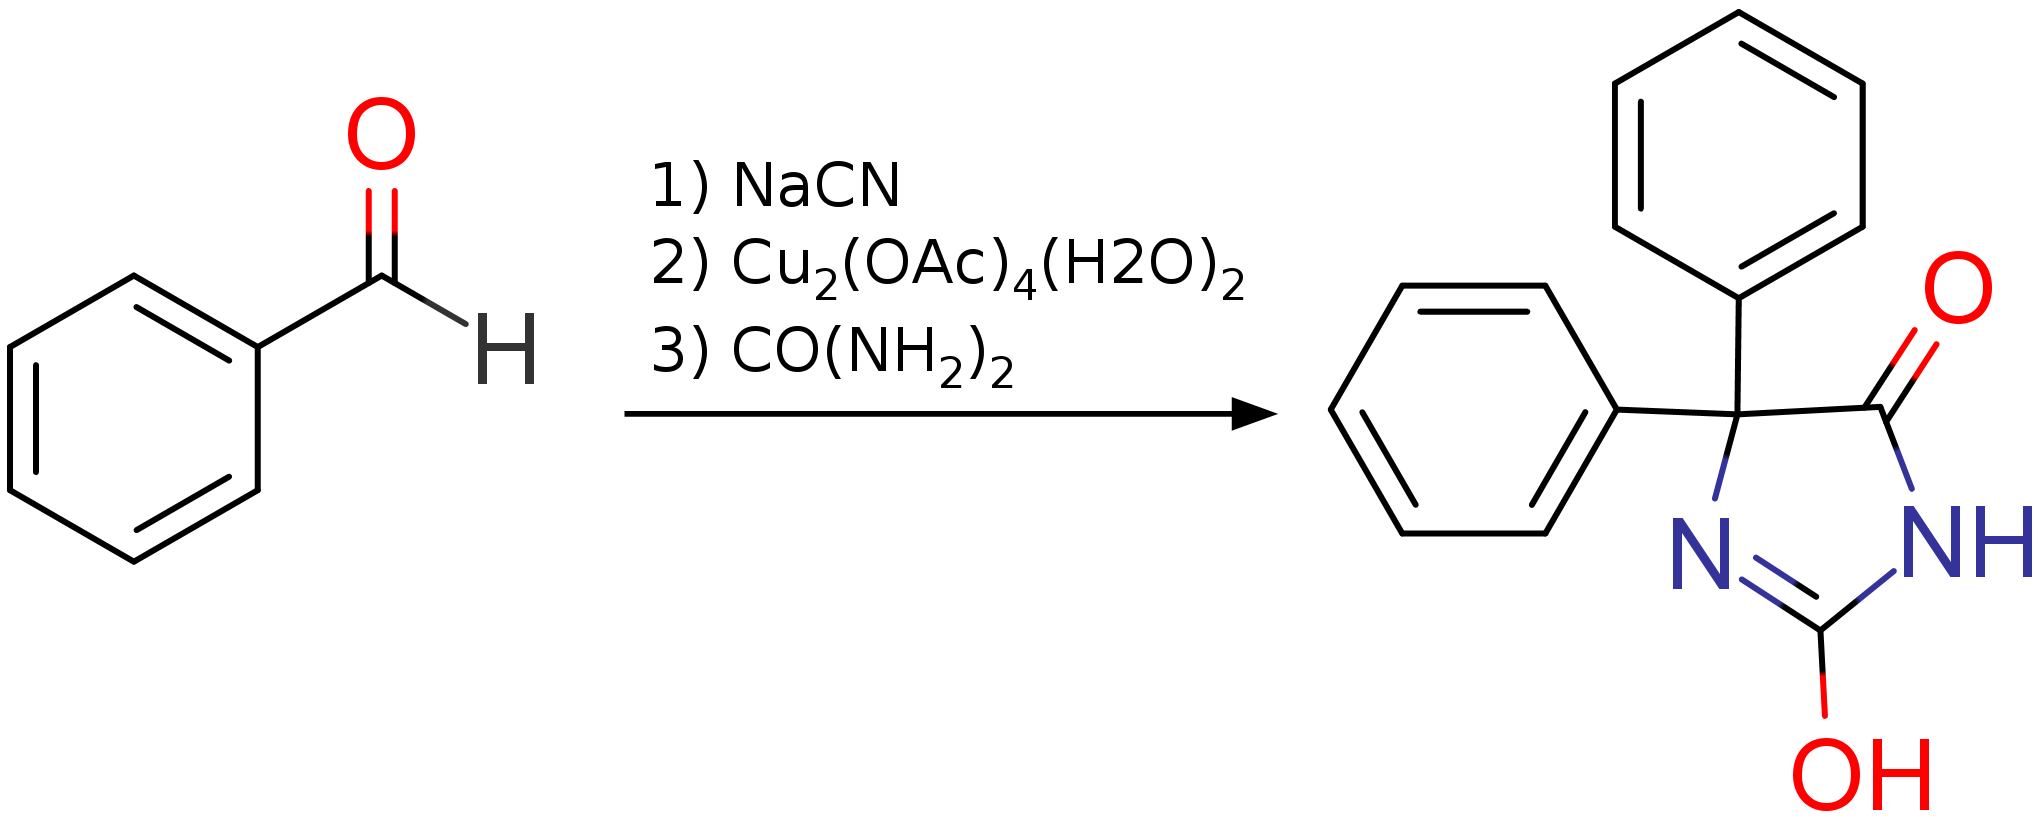
\includegraphics[scale=1]{structures/overall.png}
%\end{wrapfigure}
}

%----------------------------------------------------------------------------------------

\begin{document}

\flushbottom % Makes all text pages the same height

\maketitle % Print the title and abstract box

%\tableofcontents % Print the contents section

\thispagestyle{empty} % Removes page numbering from the first page



%----------------------------------------------------------------------------------------
%	ARTICLE CONTENTS
%----------------------------------------------------------------------------------------

\section*{Introducci\'on} % The \section*{} command stops section numbering

La triboluminiscencia es un fen\'omeno electromagn\'etico donde se obtiene emisi\'on de luz producto de estr\'es mec\'anico sobre un material. El fen\'omeno fue descubierto en 1605, sin embargo a pesar de ser estudiado por varios siglos y en procesos tan variados como el rompimiento de los cristales de azucar, la cristalizaci\'on de algunas sustancias \cite{weiser_1917}, hasta la emisi\'on inducida por laser de ondas de choque sobre un s\'olido \cite{tsuboi_seto_kitamura_2008}, contin\'ua siendo un enigma en la teor\'ia. Experimentalmente la luz emitida es caracterizada por espectroscop\'ia, de donde se ha podido concluir que el nitr\'ogeno se encuentra involucrado en varios de los procesos antes mencionados. La causa de la emisi\'on se relaciona con el movimiento de cargas el\'ectricas en una mol\'ecula cuyos enlaces qu\'imicos son modificados producto de una fuerza externa \cite{olawale_okoli_fontenot_hollerman_2016}.

Dependiendo de la topolog\'ia de la fuerza aplicada, la triboluminiscencia se divide en tres categor\'ias: el\'astica, pl\'astica y de fractura, siendo la \'ultima la estudiada en el presente documento. Estos procesos se caracterizan por el movimiento de cargas, en donde la carga de las superficies fracturadas es neutralizada por portadores de carga como iones \cite{olawale_okoli_fontenot_hollerman_2016}. 

Muchas de las sustancias que presentan este fen\'omeno contienen dopantes que modifican la energ\'ia de las bandas del s\'olido. Al reducirse la energ\'ia entre las bandas de conducci\'on y valencia del mismo se aumenta la probabilidad de emisi\'on, haciendo de estas sustancias materiales atractivos para detectores \cite{sage_humberstone_oswald_lloyd_bourhill_2001} \cite{olawale_okoli_fontenot_hollerman_2016}.

%------------------------------------------------

\section{Resultados y Discusi\'on}
La preparaci\'on del complejo triboluminiscente de cobre se realiza en dos partes. La primera es la obtenci\'on del isotiocianato de cobre (I), lo cual se realiza a partir de tiocianato de potasio y sulfato de cobre en soluci\'on. En este punto se pueden formar dos productos, la sal de cobre (II) y la de cobre (I). La primera se produce r\'apidamente dado que no involucra cambios en los estados de oxidaci\'on de los reactivos \cite{tykodi_1991}\cite{tudela_1993}.
\begin{equation}
	\ce{Cu^{2+} (ac) + 2SCN- (ac) -> [Cu(NCS)2(s)]}
\end{equation}

A pesar que el cobre (II) es el ion m\'as estable y abundante en soluci\'on, el compuesto anterior resulta poco estable debido a que su descomposici\'on da lugar a la formaci\'on de tiocian\'ogeno \ce{(SCN)2} el cual a su vez reacciona con agua dando lugar a 3 compuestos estables: \'acido tiocianico, \'acido sulf\'urico y \'acido cianh\'idrico, donde el \'ultimo se libera en forma gaseosa, desplazando el equilibrio hacia los productos \cite{tudela_1993}.

\footnotesize
\begin{equation}
	\begin{array}{c}
		\ce{[Cu(NCS)2(s)] <=>> [Cu(NCS)(s)] + (SCN)2(ac)}\\
		\ce{3(SCN)2(ac) + 4H2O(l) <=>> 5HNCS(l) + H2SO4(l) + HCN(g)}
	\end{array}
\end{equation}
\normalsize
\\

La reacci\'on anterior explica por qu\'e la descomposici\'on tiene lugar \'unicamente en soluci\'on y no como s\'olido seco. Adicionalmente permite entender el efecto de la temperatura como facilitadora de la conversi\'on del isotiocianato de cobre (II) al (I), dada la formaci\'on de un gas. Por otro lado, la concentraci\'on juega un papel importante en la formaci\'on del compuesto con deseado. Raz\'on por la cual el tiocianato fue agregado por goteo sobre la soluci\'on de cobre, logrando de esta forma que el producto obtenido tenga una relaci\'on 1:1.

Por otro lado es importante tener en cuenta que el ani\'on \ce{NCS-} tiene dos formas de enlazarse a otro \'atomo: por un lado con el nitr\'ogeno, por el otro con el azufre. En el caso del cobre el enlace tiene lugar con el nitr\'ogeno debido a la mayor al caracter intermedio del cobre y nitr\'ogeno como \'acidos y bases de Pearson.
\begin{scheme}
	\caption{Preparaci\'on del complejo \ce{[Cu(NCS)(py)2(PPh3)]}.}
	\centering
	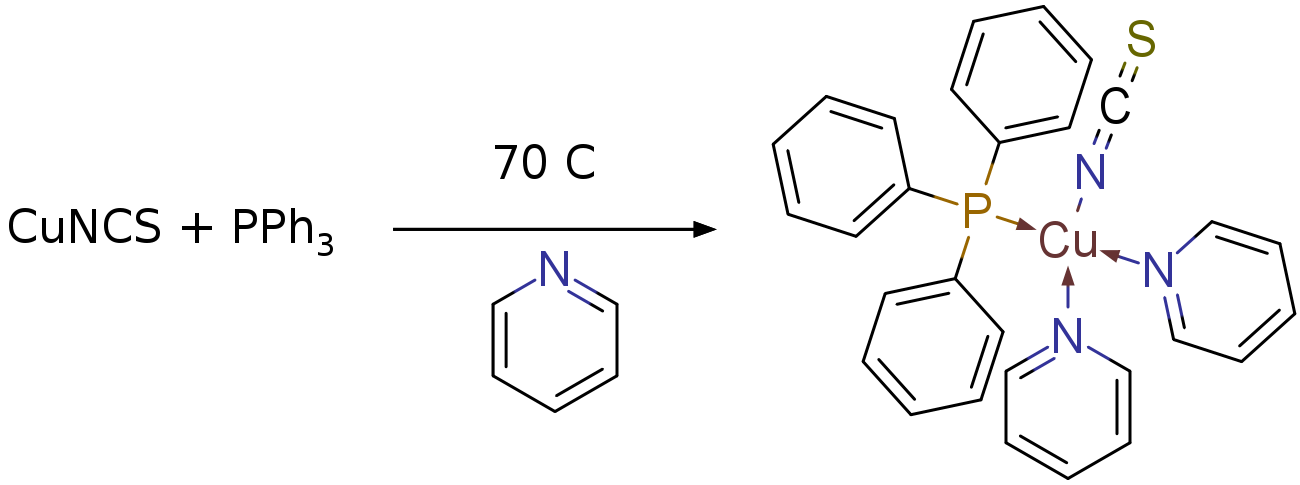
\includegraphics[width=0.8\linewidth]{Structures/tribo.png}
\end{scheme}

La segunda reacci\'on llevada a cabo es la adici\'on al centro met\'alico de dos mol\'eculas de piridina y una de trifenilfosfina, los cuales dan lugar al \ce{[Cu(NCS)(py)2(PPh3)]}, el cual presenta una geometr\'ia tetra\'edrica distorcionada por el volumen de los ligandos. La reacci\'on es netamente coordinativa donde el f\'osforo y los nitr\'ogenos de las piridinas actuan usando sus pares libres de electrones para enlazarse con el metal.

Dado que la triboluminiscencia es de fractura es necesario el rompimiento de un enlace en el cristal. Al tener en cuenta la teor\'ia propuesta por Ahrland en 1958, en donde se clasifican los cationes seg\'un su tipo: A para los m\'as livianos y de alto estado de oxidaci\'on, y B para los m\'as pesados con estados de oxidaci\'on bajos, se observa que para el caso del cobre (I) los enlaces con f\'osforo son los m\'as estables. El enlace Cu(I)-N tiene menor tendencia a formarse y por lo tanto mayor tendencia a romperse \cite{ahrland_chatt_davies_1958}. De esta forma es posible que el enlace a romperse pueda ser el de una piridina o el de isotiocianato.

Como fue comentado en la introducci\'on, la presencia de un i\'on es necesaria para la estabilizaci\'on de las nuevas superficies \cite{olawale_okoli_fontenot_hollerman_2016}\cite{marchetti_di_nicola_pettinari_timokhin_pettinari_2012}. El \'unico ligando cuya salida implicar\'ia la formaci\'on de un cati\'on met\'alico y un ani\'on es el isotiocianato. En ese sentido el rompimiento del enlace implicar\'ia la acumulaci\'on de cargas positivas y negativas en caras opuestas. El esfuerzo mec\'anico incluye la separaci\'on de las mismas, ocasionando el surgimiento de un campo el\'ectrico entre las superficies. Los campos el\'ectricos pueden de acelerar las cargas que se encuentren bajo su efecto, los electr\'ones del ani\'on pueden alcanzar velocidades tales que ionicen el medio circundante \cite{olawale_okoli_fontenot_hollerman_2016}. Los iones del medio pueden a su vez incrementar el campo o el n\'umero de choques ionizantes, generando una reacci\'on en cadena similar a la que ocurre en una descarga el\'ectrica en un rel\'ampago. 


\section{Conclusiones}

\section{Secci\'on experimental}
\subsection{S\'intesis de \ce{[Cu(NCS)(py)2(PPh3)]}}
La preparaci\'on de las sales se realiza usando dos soluciones 0.25 M (1.0 eq) de tiocianato de potasio y sulfato de cobre anhidro. Sobre un bal\'on con 25 mL de la soluci\'on de sulfato de cobre son adicionados 25 mL de la soluci\'on de tiocianato por goteo. La reacci\'on se calienta y agita por media hora, posteriormente se filtra el producto al vac\'io. Una mezcla con 0.2526 g ( eq) de tiocianato de cobre (I) y 0.5300 g ( eq) de trifenilfosfina se disuelve en 10 mL de piridina. La reacci\'on se lleva a cabo en reflujo por 3 horas.

\subsection{Reducci\'on con nanopart\'iculas}
Una soluci\'on tetrahidroborato de sodio (\ce{NaBH4}) se prepara con la disoluci\'on de 0.080 g del mismo en 10 mL de agua. Se prepara una segunda soluci\'on con 0.259 g de polivinilpirrolidina junto con 0.100 g de cloruro de cobalto hexahidratado en 10 mL de agua. La soluci\'on de \ce{NaBH4} se adiciona por goteo en presencia de ultrasonido. El producto obtenido se separa en dos mitades, una de las cuales se hace reaccionar con 0.1504 g de \textit{p}-nitrobenzaldehido y 0.2 mL de hidracina hidratada. La reacci\'on se sigue por cromatograf\'ia de placa delgada, usando diclorometano. El producto se obtiene por evaporaci\'on a presi\'on reducida luego de 90 minutos del inicio de la reacci\'on.

\subsection{S\'intesis de un cluster termocr\'omico}
Tres soluciones acuosas con vol\'umenes 15 mL, 30 mL y 10 mL son preparadas. La primera contiene 1.6205 g de sulfato de cobre pentahidratado, la segunda 0.5000 g de sulfito de sodio y la tercera 1.0800 g de yoduro de potasio. Sobre la segunda soluci\'on se adiciona \'acido sulf\'urico concentrado y se mezcla con la primera. Una vez disueltos los s\'olidos se adiciona la \'ultima soluci\'on a la mezcla. El yoduro de cobre obtenido se agrega a una soluci\'on 0.52 mL de piridina y 5 mL de acetonitrilo, sobre la misma se adicionan 0.7726 g de yoduro de potasio y 0.0332 g de \'acido asc\'orbico. La soluci\'on se agita por 15 minutos, posterior a los cuales se adicionan 25 mL de agua. El producto se filtra al vac\'io.  

%----------------------------------------------------------------------------------------
%	REFERENCE LIST
%----------------------------------------------------------------------------------------
\phantomsection
\bibliography{informe}
\bibliographystyle{unsrt}

%----------------------------------------------------------------------------------------
\newpage
\onecolumn
\section{Informaci\'on suplementaria}\label{sec: complementaria}

\end{document}